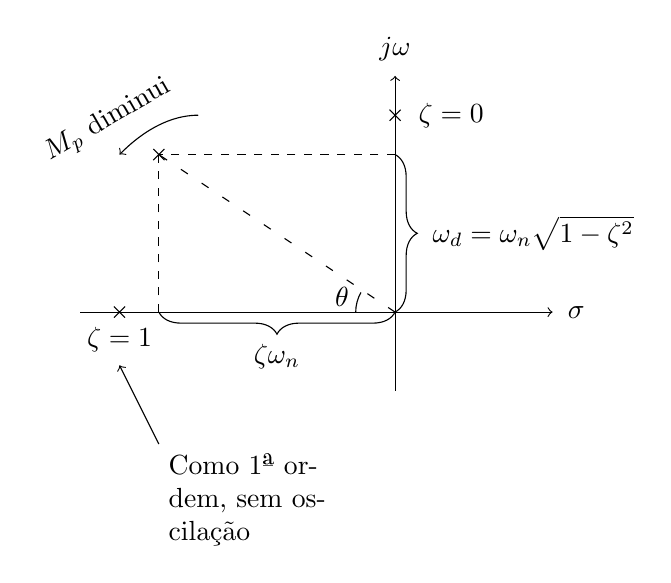
\begin{tikzpicture}
\draw[->] (-4,0) -- (2,0) node[right=2pt] {$ \sigma $};
\draw[->] (0,-1) -- (0,3) node[above=2pt] {$ j\omega $};

\draw[dashed] (-3,0) -- (-3,2);

\draw[dashed] (0,2) -- (-3,2);

\draw[loosely dashed] (0,0) -- (-3,2);
\draw (-3,2) ++(-2pt,-2pt) -- ++(4pt,4pt) ++(-4pt,0pt) -- +(4pt,-4pt);

\draw[->] (-2.5,2.5) parabola (-3.5,2) node[above=5pt, rotate=30] {$ M_p $ diminui};

\draw (0,2.5) node[right=5pt] {$ \zeta=0 $} ++(-2pt,-2pt) -- ++(4pt,4pt) ++(-4pt,0pt) -- +(4pt,-4pt);

\draw (-0.5,0) arc (180:150:0.5) node[left,near end] {$ \theta $};

\draw (-3.5,0) node[below=2pt] {$ \zeta=1 $} ++(-2pt,-2pt) -- ++(4pt,4pt) ++(-4pt,0pt) -- +(4pt,-4pt);

\draw[<-] (-3.5,-0.5) ++(0,-5pt) -- +(0.5,-1) node[below right, text width=2.5cm] {Como 1ª ordem, sem oscilação};

\draw[decorate,decoration={brace,amplitude=8pt}, xshift=0] (0,2) -- node[right=10pt] {$ \omega_d=\omega_n\sqrt{1-\zeta^{2}} $} (0,0) ;

\draw[decorate,decoration={brace,amplitude=8pt}, xshift=0] (0,0) -- node[below=8pt] {$ \zeta\omega_n $} (-3,0) ;
\end{tikzpicture}
